\documentclass[10pt]{article}

\def\Type{LessonCaelan}
\def\TypeNum{Lesson 21}
\def\TypeTitle{Continuous Random Variables}
\def\Semester{Fall 2021} %Not Used 
\def\Course{MATH 1190 \& 1210}

\usepackage{preambleDJ}



%%%%%%%%%%%% BEGIN DOCUMENT %%%%%%%%%%%%%%%
%%%%%%%%%%%% BEGIN DOCUMENT %%%%%%%%%%%%%%%
%%%%%%%%%%%% BEGIN DOCUMENT %%%%%%%%%%%%%%%
%%%%%%%%%%%% BEGIN DOCUMENT %%%%%%%%%%%%%%%
%%%%%%%%%%%% BEGIN DOCUMENT %%%%%%%%%%%%%%%

\begin{document}


\thispagestyle{firstpage}
\pagestyle{otherpages}
\vs{0.4}

%\Heading{MATH 1190 \& 1210 Survey of Calculus I}{\begin{minipage}{0.25\textwidth}\begin{center} Lesson 20\\ Introduction to Probability \end{center}\end{minipage}}

\textbf{Intended Learning Outcomes}
After this lesson, you will be able to 

\begin{itemize}
    \item Determine if a random variable is discrete or continuous. (\target{P2})
    \item Define support for a continuous random variable. (\target{P2})
    \item List and apply properties of the probability density function of a continuous random variable. (\target{P2})
    \item Find the formula and the graph of the cumulative distribution function of a continuous random variable. (\target{P2)}
\end{itemize}

\vspace{-0.5cm}

\hrulefill

\textbf{\color{blue} Warm Up}\exercise{\bf\color{Orange}P2} Determine whether each of the random variable in the following scenarios is discrete or continuous.

\begin{enumerate}[label=(\alph*)]
    \item The number of arrivals at an emergency room from midnight to 6am on a given day.

    \vfill

    \item The temperature of a cup of coffee from a coffee shop.

    \vfill 

    \item The number of boys in a randomly-selected family with 3 children.

    \vfill
\end{enumerate}

%%%%%%%%%
\newpage%
%%%%%%%%%

{\bf\color{blue}Mini-lecture.} ({\it Smoothing out the Age Historgram})

\begin{center}
    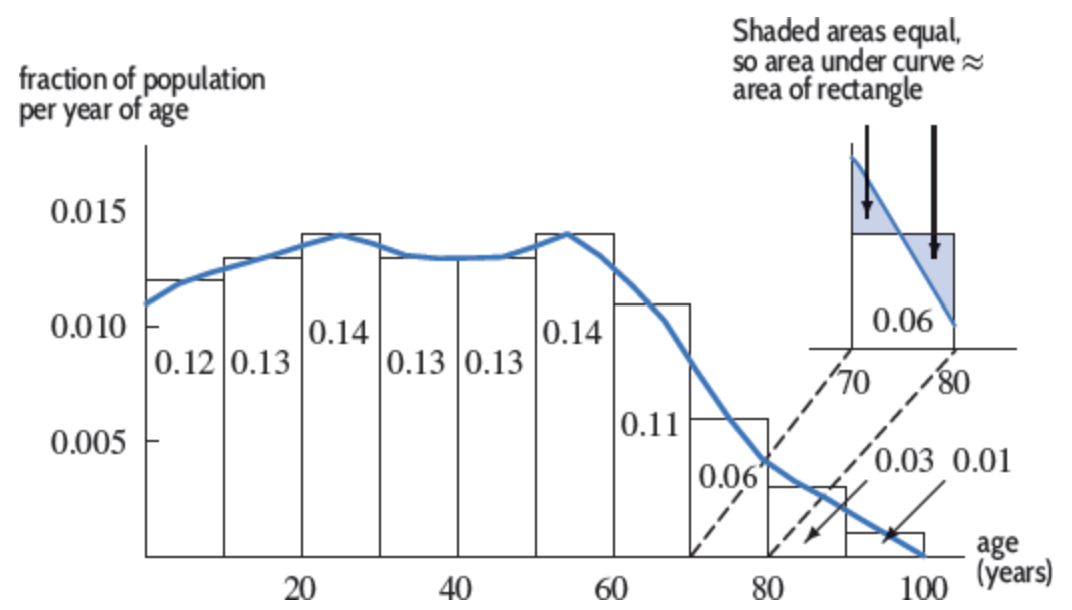
\includegraphics[scale=0.8]{agehistogram.png}
\end{center}

Suppose $t$ is age in years. We define $p(t)$, the \textbf{probability} density function for age, to be the function that "smoothes out" the age histogram.

If $a$ and $b$ are two ages such that $b\ge a$, then

\[\text{percentage of Population between age $a$ and age $b$}=\int_a^b p(t)\,dt.\]

If the smallest possible age is $0$ and largest possible age is $100$, then 

\[\int_0^{100} p(t)\,dt=1.\]

\fbox{
\begin{minipage}{0.95\textwidth}
\textbf{The Probability Density Function, Properties, and Support}

More generally, for a continuous random variable $X$, its \textbf{probability density function} (PDF) $p(x)$ satisfies that 

\[P(a<X<b)=\int_a^bp(x)\,dx.\]

Analogous to the probability mass function, any probability density function $p(x)$ satisfy the following two important properties.

\begin{enumerate}
    \item For all real numbers $x$, the value of $p(x)$ is always non-negative.
    \item If $a$ is the smallest possible value of $x$ where $p(x)>0$, and $b$ is the largest possible value of $x$ where $p(x)>0$, then 
    \[\int_a^b p(x)\,dx=1.\]
\end{enumerate}

The \textbf{support} of a continuous random variable \(X\) is the smallest interval that contains all number that gives a positive value of the probability density function of \(X\).

\end{minipage}
}

\example{\bf\color{Orange}P2} A person arrives at a bus stop at a random time to catch the next bus. Buses run every 30 minutes without fail, hence the next bus could come any time during the next 30 minutes with evenly distributed probability (a uniform distribution).

Suppose $X$ represents the number of minutes this person waits until the next bus arrives.

\begin{enumerate}[label=(\alph*)]
    \item What is the support of $X$?

    \vfill

    \newpage

    \item Sketch the graph of the probability density function $p(x)$ of $X$, and find its formula using the properties of the probability density function.

    \vfill

    \item Use $p(x)$ and an integral to find the probability that this person waits for no more than 10 minutes.

    \vfill
\end{enumerate}

\exercise{\bf\color{Orange}P2}
Let $X$ be a continuous random variable with probability density function given by:
\[
p(x) = 
\begin{cases} 
cx & \text{for } 0 \leq x \leq 2, \\
0 & \text{otherwise}.
\end{cases}
\]
\begin{itemize}

\item[(a)] Find the support of $X$.
%
\,\hfill
{\large
$\rule[-2pt]{2in}{0.4pt}$
}
\hfill\,

\item[(b)] Find the value of the constant $c$ making $p(x)$ a valid probability density function. Then sketch $p(x)$ within the support of $X$.

\vfill

\item[(c)] Using the value of $c$ you found, find the probability that $X$ takes on a value less than or equal to $1.5$.

\vfill

\item[(d)] Find an interval $[0,b]$ that $X$ has a $25\%$ chance of falling in. Show your answer is correct.

\vfill

\end{itemize}

%%%%%%%%%
\newpage%
%%%%%%%%%

{\bf\color{blue}Mini-lecture.} Suppose the support of a continuous random variable $X$ is $[a, b]$. The {\bf cumulative distribution function} (CDF) of $X$ is given by
\[C(x) = \rule[-8pt]{2in}{0.4pt},\] for $a\le x\le b$.

In contrast, the PDF and the CDF are also related in the following way. \[p(x)=C'(x)\]

The CDF of a random variable measures how much probability has accumulated up to a given point. It has the following properties.
\begin{enumerate}
    \item $C(x)$ is always non-negative.
    \item $C(x)$ never decreases.
    \item $C(x)=0$ when $x<a$ and $C(x)=1$ when $x>b$.
    \item Assume $c$ and $d$ are within the support of $X$ with $c<d$. The probability of the value of $X$ falls into some interval $(c, d)$ is $C(d)-C(c)$.
\end{enumerate}



\example{\bf\color{Orange}P2} Let's continue with Example 1. Based on the definition we just learned, what is the cumulative distribution function of the random variable $X$ in this scenario? Find its formula and sketch its graph.

\vfill

\exercise{\bf\color{Orange}P2}
The PDF of the continuous random variable $X$ is given below:\\

\

\,\hfill
%
\begin{minipage}[t][0.5in]{0.25\textwidth}
$
p(x) = 
\begin{cases} 
1 & \text{for } 0 \leq x \leq 1, \\
0 & \text{otherwise},
\end{cases}
$
\end{minipage}
%
\hfill
%
\begin{minipage}[t][0.5in]{0.25\textwidth}
\,\\[-0.5in]
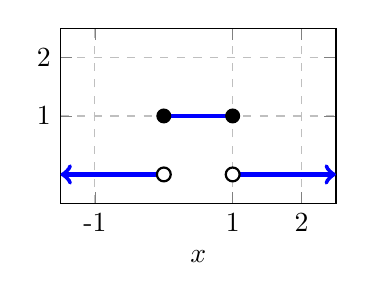
\begin{tikzpicture}
          \begin{axis}[
        %    axis y line = left,
        %    axis x line = bottom,
            xlabel = {$x$},
            xtick       = {-1,1,2},
            xticklabels = {-1,1,2},
            ytick       = {1,2},
            yticklabels = {1,2},
            samples     = 160,
            domain      = -1:3,
            restrict y to domain=-0.1:4,
            xmin = -1.5, xmax = 2.5,
            ymin = -0.5, ymax = 2.5,
            width = 2in, height=1.5in,
            grid=both, grid style=dashed
          ]
          \draw[ultra thick,blue,<-] (-1.5,0) -- (0,0);
          \draw[ultra thick,blue] (0,1) -- (1,1);
          \draw[ultra thick,blue,->] (1,0) -- (2.5,0);
          \filldraw (0,1) circle (2.5pt);
          \filldraw (1,1) circle (2.5pt);
          \filldraw[fill=white, thick] (1,0) circle (2.5pt);
          \filldraw[fill=white, thick] (0,0) circle (2.5pt);
        \end{axis}
\end{tikzpicture}
\end{minipage}
%
\hfill\,\\

\begin{itemize}
\item[(a)] Use the formula in the mini-lecture to find the CDF $C(x)$ of $X$.

\vfill

\end{itemize}

\begin{minipage}[t]{0.5\textwidth}
\begin{itemize}
\item[(b)] Sketch the part of the graph of the CDF $C(x)$ within the support of $X$.

    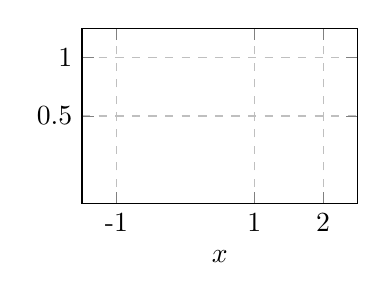
\begin{tikzpicture}
          \begin{axis}[
        %    axis y line = left,
        %    axis x line = bottom,
            xlabel = {$x$},
            xtick       = {-1,1,2},
            xticklabels = {-1,1,2},
            ytick       = {1,2},
            yticklabels = {0.5,1},
            samples     = 160,
            domain      = -1:3,
            restrict y to domain=-0.1:4,
            xmin = -1.5, xmax = 2.5,
            ymin = -0.5, ymax = 2.5,
            width = 2in, height=1.5in,
            grid=both, grid style=dashed
          ]
        \end{axis}
    \end{tikzpicture}
\end{itemize}
\end{minipage}
%
\begin{minipage}[t]{0.45\textwidth}
    \begin{itemize}
    \item[(c)] Find the number $m$ for which $P(X<m)=0.5$. ({\bf Note:} this number $m$ is called the {\bf median} of $X$.)
    \end{itemize}
\end{minipage}\\

%%%%%%%%%
\newpage%
%%%%%%%%%

\exercise{\bf\color{Orange}P2} Let $X$ be a continuous random variable. The following graph is either the graph of the PDF $p(x)$ or the CDF $C(x)$.

\begin{center}
     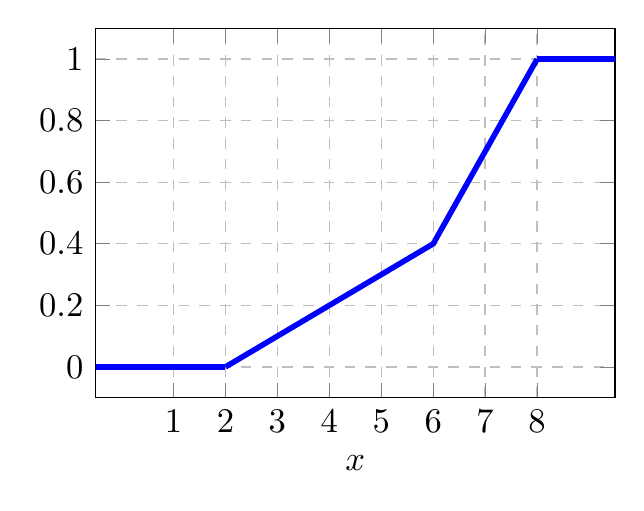
\begin{tikzpicture}[scale=1.25]
           \begin{axis}[
             xlabel={$x$},
             %grid = major,
             xtick       = {1,2,3,4,5,6,7,8},
             xticklabels = {$1$,$2$,$3$,$4$,$5$,$6$,$7$,$8$},
             ytick       = {0, 0.2, 0.4, 0.6, 0.8, 1},
             yticklabels = {$0$, $0.2$, $0.4$, $0.6$, $0.8$, $1$},
             samples     = 320,
             domain      = -1:9.5,
             restrict y to domain=-3.5:2.5,
             xmin = -0.5, xmax = 9.5,
             ymin = -0.1, ymax = 1.1,
             height=2.1in, width=2.7in,
             grid=both, grid style=dashed
           ]
           \draw[ultra thick, blue,-] (2,0) -- (6, 0.4) -- (8,1);
           \draw[ultra thick, blue,-] (-0.5,0) -- (2,0);
           \draw[ultra thick, blue,-] (8, 1) -- (9.5,1);
           %\draw (2,0) circle (1.5pt);
           %\draw (8,0) circle (1.5pt);
           %\draw[blue,fill=blue] (2,0.08) circle (1.5pt);
           %\draw[blue,fill=blue] (8,0.12) circle (1.5pt);
           %\node at (3,0.2) {$p(x)$};
           \end{axis}
     \end{tikzpicture}
     \end{center}

\begin{enumerate}
    \item[(a)] Determine whether the graph is of $p(x)$ or $C(x)$, and explain why. 

    \vfill

    \item[(b)] Based on the graph, what is the probability that the value of $X$ falls between 4 and 6?

    \vfill

    \item[(c)] What is the support of $X$?

    \vfill

    \item[(d)] Find the formula or the graph of the PDF $p(x)$ or the CDF $C(x)$, which ever is NOT represented by the given graph.

    \vfill
\end{enumerate}

% \exercise{\bf\color{Orange}P2}
% Suppose we want to analyze the fishing industry in a small town. Each day, the boats bring back at least 2 tons of fish, but never more than 8 tons.

% Suppose $X$ is the continuous random variable for the amount of fish brought back by the boats on a day. The following figure shows the the probability density function $p(x)$ of $X$. 

% \begin{center}
%     \begin{tikzpicture}[scale=1.25]
%           \begin{axis}[
%             xlabel={$x$},
%             %grid = major,
%             xtick       = {1,2,3,4,5,6,7,8},
%             xticklabels = {$1$,$2$,$3$,$4$,$5$,$6$,$7$,$8$},
%             ytick       = {0, 0.04, 0.08, 0.12, 0.16, 0.2, 0.24, 0.28},
%             yticklabels = {$0$, , $0.08$, $0.12$, ,,$0.24$, ,},
%             samples     = 320,
%             domain      = -1:9.5,
%             restrict y to domain=-3.5:2.5,
%             xmin = -0.5, xmax = 9.5,
%             ymin = -0.1, ymax = 0.3,
%             height=2.1in, width=2.7in,
%             grid=both, grid style=dashed
%           ]
%           \draw[ultra thick, blue,-] (2,0.08) -- (6,0.24) -- (8,0.12);
%           \draw[ultra thick, blue,-] (-0.5,0) -- (1.95,0);
%           \draw[ultra thick, blue,-] (8.05,0) -- (9.5,0);
%           \draw (2,0) circle (1.5pt);
%          \draw (8,0) circle (1.5pt);
%           \draw[blue,fill=blue] (2,0.08) circle (1.5pt);
%           \draw[blue,fill=blue] (8,0.12) circle (1.5pt);
%           \node at (3,0.2) {$p(x)$};
%           \end{axis}
%     \end{tikzpicture}
%     \end{center}

% \begin{enumerate}
%     \item[(a)] Find and graph the corresponding cumulative distribution function.

%     \vfill

%     \item[(b)] What is the probability that the catch of the day is between 5 and 7 tons?

%     \vfill
% \end{enumerate}



{\bf\color{blue}Extra Practice 1.} \ltrm{\bf\color{Orange}P2}Consider the following probability density function for a random variable $X$:
\[
    p(x) = 
    \begin{cases} 
    cx(1 - x) & \text{for } 0 \leq x \leq 1, \\
    0 & \text{otherwise}.
    \end{cases}
\]
\begin{enumerate}
\item[(a)] Find the value of $c$ making $f$ a valid probability density function.
    
\vfill

\item[(b)] Suppose you know $X$ has a 75\% chance to fall in the interval $[a,1]$. Find $a$.

\vfill

%%%%%%%%%
\newpage%
%%%%%%%%%

\item[(c)] Suppose you know $X$ has a 25\% chance to fall in the interval $[0,b]$. Find $b$.

\vfill

\item[(d)] What do you notice about $a$ and $b$? How is this relationship related to the fact that $\displaystyle\int_0^1 p(x)\,dx$ must equal $1$? ({\bf Hint:} you might want to use a property of definite integrals to explain your answer.)

\vfill

\end{enumerate}

{\bf\color{blue}Extra Practice 2.} \ltrm{\bf\color{Orange}P2}
The probability density function of a random variable $X$ is given below:
\[
p(x) = 
\begin{cases} 
3x^2 & \text{for } 0 \leq x \leq 1, \\
0 & \text{otherwise},
\end{cases}
\]
Find and graph the cumulative distribution function $C(x)$.\\

\vfill

\,\hfill
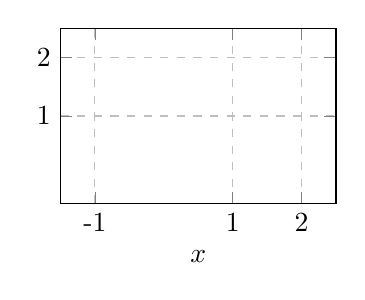
\begin{tikzpicture}
          \begin{axis}[
        %    axis y line = left,
        %    axis x line = bottom,
            xlabel = {$x$},
            xtick       = {-1,1,2},
            xticklabels = {-1,1,2},
            ytick       = {1,2},
            yticklabels = {1,2},
            samples     = 160,
            domain      = -1:3,
            restrict y to domain=-0.1:4,
            xmin = -1.5, xmax = 2.5,
            ymin = -0.5, ymax = 2.5,
            width = 2in, height=1.5in,
            grid=both, grid style=dashed
          ]
        \end{axis}
    \end{tikzpicture}







% {\bf\color{blue}Extra Practice 3.} \ltrm{\bf\color{Orange}P3}
% Consider the probability density function of the continuous random variable $Z$:
% \[
% p(z) = 
% \begin{cases} 
% \dfrac{1}{12}z & \text{for } 1 \leq z \leq 5, \\
% 0 & \text{otherwise}.
% \end{cases}
% \]
% \begin{itemize}

% \item[(a)] Find $P(2\leq Z\leq 4)$.

%     \vfill
%     \vfill
    
% \item[(b)] Find the CDF and median of $Z$.

%     \vfill
%     \vfill
%     \vfill

% \end{itemize}

\end{document}

%%%%%%%%%
\newpage%
%%%%%%%%%

\begin{center}
({\it Conditioning \& Independence})
\end{center}

\begin{itemize}
    \item If $E$ and $F$ are both events, then the {\bf intersection} $E\cap F$ of both events is the event whose outcomes are in both $E$ and $F$; in other words, $E\cap F$ is the event that both $E$ and $F$ occur.
    \item If $E$ and $F$ are both events, then the event $E|F$ is the event that $E$ occurs given the condition that $F$ has already occurred. The knowledge that an event has already occurred can change how we think about possible outcomes and thus probabilities.
    \item Two events $E$ and $F$ are called {\bf independent} if knowledge that $F$ has occurred does not change the probability that $E$ occurs; that is,
    \[P(E|F)=P(E)\]
\end{itemize}

\exercise\lt{{\bf\color{Orange}P1}} A coin is flipped three times, and the upturned face is recorded after each flip. Assume each outcome - heads or tails - is equally likely for each flip.
    \begin{itemize}
    \item[(a)] What is the sample space $S$ of this experiment?

    {\Large
    \[
    S = \rule[-8pt]{5in}{0.4pt}
    \]
    }
    
    \item[(b)] Let $E_1$ be the event that the first flip lands on heads. What is $E_1$?

    {\Large
    \[
    E_1 = \rule[-8pt]{4in}{0.4pt}
    \]
    }
    
    \item[(c)] Let $E_2$ be the event that the second flip lands on heads. What is $E_2$?

    {\Large
    \[
    E_2 = \rule[-8pt]{4in}{0.4pt}
    \]
    }

    \item[(d)] What is $E_2|E_1$? Describe $E_2|E_1$ in the given context in words, as well.

    {\Large
    \[
    E_2|E_1 = \rule[-8pt]{4in}{0.4pt}
    \]
    }

    \vfill

    \item[(e)] Find the probability that $E_1$ occurs, the probability that $E_2$ occurs, and the probability that $E_2|E_1$ occurs. Are $E_1$ and $E_2$ independent? Explain.\\

    \vfill
        
    {\large
        \,\hfill
        $P(E_1)=$\rule[-8pt]{1.25in}{0.4pt}
        \hfill
        $P(E_2)=$\rule[-8pt]{1.25in}{0.4pt}
        \hfill
        $P(E_2|E_1)=$\rule[-8pt]{1.25in}{0.4pt}
        \hfill\,\\
    }
    
    \end{itemize}

%%%%%%%%%
\newpage%
%%%%%%%%%

{\bf\color{blue}Extra Practice 3.}\lt{{\bf\color{Orange}P1}} Suppose we toss two 4-sided dice - one painted {\color{red}red} and one painted {\color{blue}blue} - and record the result as an ordered pair $(\rule[-2pt]{0.2in}{0.4pt},\rule[-2pt]{0.2in}{0.4pt})$ with the first coordinate referring to the value of the {\color{red}red} die and the second coordinate referring to the value of the {\color{blue}blue} die. Assume each outcome - 1, 2, 3, or 4 - is equally likely for both dice.
    \begin{itemize}
    \item[(a)] Fill in the sample space $S$:

    {\Large 
    \begin{align*}
    S = \bigg\{ &\big( \rule[-4pt]{0.5in}{0.4pt}, \rule[-4pt]{0.5in}{0.4pt} \big), \, \big( \rule[-4pt]{0.5in}{0.4pt}, \rule[-4pt]{0.5in}{0.4pt} \big), \, \big( \rule[-4pt]{0.5in}{0.4pt}, \rule[-4pt]{0.5in}{0.4pt} \big), \, \big( \rule[-4pt]{0.5in}{0.4pt}, \rule[-4pt]{0.5in}{0.4pt} \big),\\[0.1in]
    &\big( \rule[-4pt]{0.5in}{0.4pt}, \rule[-4pt]{0.5in}{0.4pt} \big), \, \big( \rule[-4pt]{0.5in}{0.4pt}, \rule[-4pt]{0.5in}{0.4pt} \big), \, \big( \rule[-4pt]{0.5in}{0.4pt}, \rule[-4pt]{0.5in}{0.4pt} \big), \, \big( \rule[-4pt]{0.5in}{0.4pt}, \rule[-4pt]{0.5in}{0.4pt} \big),\\[0.1in]
    &\big( \rule[-4pt]{0.5in}{0.4pt}, \rule[-4pt]{0.5in}{0.4pt} \big), \, \big( \rule[-4pt]{0.5in}{0.4pt}, \rule[-4pt]{0.5in}{0.4pt} \big), \, \big( \rule[-4pt]{0.5in}{0.4pt}, \rule[-4pt]{0.5in}{0.4pt} \big), \, \big( \rule[-4pt]{0.5in}{0.4pt}, \rule[-4pt]{0.5in}{0.4pt} \big),\\[0.1in]
    &\big( \rule[-4pt]{0.5in}{0.4pt}, \rule[-4pt]{0.5in}{0.4pt} \big), \, \big( \rule[-4pt]{0.5in}{0.4pt}, \rule[-4pt]{0.5in}{0.4pt} \big), \, \big( \rule[-4pt]{0.5in}{0.4pt}, \rule[-4pt]{0.5in}{0.4pt} \big), \, \big( \rule[-4pt]{0.5in}{0.4pt}, \rule[-4pt]{0.5in}{0.4pt} \big) \bigg\}
    \end{align*}
    }

    \item[(b)] Let $E$ be the event that the sum of the displayed values is at least $7$. What is $E$? What is $P(E)$?

    {\Large
    \[
    E = \rule[-8pt]{4in}{0.4pt} \quad \& \quad P(E) = \rule[-8pt]{1in}{0.4pt}
    \]
    }

    \item[(c)] %By accident, we toss the dice so that one of the dice falls off the table onto which we tossed the dice initially, obscuring its value from our view. On the table, however, we see that the red die displays $4$.
    Let $F$ be the event that the {\color{red}red} die displays $4$. What is $F$? What is $P(F)$?

    {\Large
    \[
    F = \rule[-8pt]{4in}{0.4pt} \quad \& \quad P(F) = \rule[-8pt]{1in}{0.4pt}
    \]
    }
    \item[(d)] Describe $E|F$ in the given context in words. What is $E|F$ as a set?

    \vfill

    {\Large
    \[
    E|F = \rule[-8pt]{4in}{0.4pt}
    \]
    }
    \item[(e)] Find $P(E|F)$, and decide whether $E$ and $F$ are independent events.
    
    \vfill
    
    {\Large \hfill $P(E|F)=\rule[-8pt]{1in}{0.4pt}$}
    \end{itemize}
%%%%%%%%%%%%%%%%
\newpage
%%%%%%%%%%%%%%
{\bf\color{blue}Extra Practice 4.}\lt{{\bf\color{Orange}P1}} Many board games use strange dice. Suppose in one such game we toss one standard six-sided die and one four-sided die in a game. Assume each outcome - 1, 2, 3, 4, 5, or 6 - is equally likely for the six-sided die and each outcome 1, 2, 3, or 4 is equally likely for the four-sided die. Further, lets suppose we always roll the six-sided die first and the four-sided die second.

    \begin{itemize}
    \item[(a)] Fill in the sample space $S$:
     \begin{align*}
    S = \bigg\{
        &(\rule[-4pt]{0.3in}{0.4pt}, \rule[-4pt]{0.3in}{0.4pt}), \, (\rule[-4pt]{0.3in}{0.4pt}, \rule[-4pt]{0.3in}{0.4pt}), \, (\rule[-4pt]{0.3in}{0.4pt}, \rule[-4pt]{0.3in}{0.4pt}), \, (\rule[-4pt]{0.3in}{0.4pt}, \rule[-4pt]{0.3in}{0.4pt}), \, (\rule[-4pt]{0.3in}{0.4pt}, \rule[-4pt]{0.3in}{0.4pt}), \, (\rule[-4pt]{0.3in}{0.4pt}, \rule[-4pt]{0.3in}{0.4pt}) \\[5pt]
        &(\rule[-4pt]{0.3in}{0.4pt}, \rule[-4pt]{0.3in}{0.4pt}), \, (\rule[-4pt]{0.3in}{0.4pt}, \rule[-4pt]{0.3in}{0.4pt}), \, (\rule[-4pt]{0.3in}{0.4pt}, \rule[-4pt]{0.3in}{0.4pt}), \, (\rule[-4pt]{0.3in}{0.4pt}, \rule[-4pt]{0.3in}{0.4pt}), \, (\rule[-4pt]{0.3in}{0.4pt}, \rule[-4pt]{0.3in}{0.4pt}), \, (\rule[-4pt]{0.3in}{0.4pt}, \rule[-4pt]{0.3in}{0.4pt}) \\[5pt]
        &(\rule[-4pt]{0.3in}{0.4pt}, \rule[-4pt]{0.3in}{0.4pt}), \, (\rule[-4pt]{0.3in}{0.4pt}, \rule[-4pt]{0.3in}{0.4pt}), \, (\rule[-4pt]{0.3in}{0.4pt}, \rule[-4pt]{0.3in}{0.4pt}), \, (\rule[-4pt]{0.3in}{0.4pt}, \rule[-4pt]{0.3in}{0.4pt}), \, (\rule[-4pt]{0.3in}{0.4pt}, \rule[-4pt]{0.3in}{0.4pt}), \, (\rule[-4pt]{0.3in}{0.4pt}, \rule[-4pt]{0.3in}{0.4pt}) \\[5pt]
        &(\rule[-4pt]{0.3in}{0.4pt}, \rule[-4pt]{0.3in}{0.4pt}), \, (\rule[-4pt]{0.3in}{0.4pt}, \rule[-4pt]{0.3in}{0.4pt}), \, (\rule[-4pt]{0.3in}{0.4pt}, \rule[-4pt]{0.3in}{0.4pt}), \, (\rule[-4pt]{0.3in}{0.4pt}, \rule[-4pt]{0.3in}{0.4pt}), \, (\rule[-4pt]{0.3in}{0.4pt}, \rule[-4pt]{0.3in}{0.4pt}), \, (\rule[-4pt]{0.3in}{0.4pt}, \rule[-4pt]{0.3in}{0.4pt}) 
    \bigg\}
       \end{align*}
    

    \item[(b)] Lets suppose that you are in a position to win the game, but the sum of the numbers on the upturned faces of your next dice roll must be at least $8$. Let $E$ be the event that the sum of the displayed values on your next roll is at least $8$. What is $E$? What is $P(E)$?

    {\Large
    \[
    E = \rule[-8pt]{4in}{0.4pt} \quad \& \quad P(E) = \rule[-8pt]{1in}{0.4pt}
    \]
    }

    \item[(c)] %By accident, we toss the dice so that one of the dice falls off the table onto which we tossed the dice initially, obscuring its value from our view. On the table, however, we see that the red die displays $4$.
    Let $F$ be the event that the four-sided die displays $2$. What is $F$ as an set? What is $P(F)$?

    {\Large
    \[
    F = \rule[-8pt]{4in}{0.4pt} \quad \& \quad P(F) = \rule[-8pt]{1in}{0.4pt}
    \]
    }
    \item[(d)] %By accident, we toss the dice so that one of the dice falls off the table onto which we tossed the dice initially, obscuring its value from our view. On the table, however, we see that the red die displays $4$.
    Let $G$ be the event that the four-sided die displays $4$. What is $G$ as an set? What is $P(G)$?

    {\Large
    \[
    G = \rule[-8pt]{4in}{0.4pt} \quad \& \quad P(G) = \rule[-8pt]{1in}{0.4pt}
    \]
    }
    \item[(e)] Describe $E|F$ in the given context in words. What is $E|F$ as a set?
    \vspace{3in}

    \vfill

    {\Large
    \[
    E|F = \rule[-8pt]{4in}{0.4pt}
    \]
    }
    \item[(f)] Describe $E|G$ in the given context in words. What is $E|G$ as a set?
    \vspace{2in}

    \vfill

    {\Large
    \[
    E|G = \rule[-8pt]{4in}{0.4pt}
    \]
    }
    \item[(g)] Find $P(E|F)$, and decide whether $E$ and $F$ are independent events.

    \vfill

    {\Large \hfill $P(E|F)=\rule[-8pt]{1in}{0.4pt}$}
    \item[(h)] Find $P(E|G)$, and decide whether $E$ and $G$ are independent events.

    \vfill

    {\Large \hfill $P(E|G)=\rule[-8pt]{1in}{0.4pt}$}
    \item[(i)] Which of the two events gives you a better chance of winning, $F$ or $G$? Explain.

    \vfill

    \end{itemize}
%%%%%%%%%
\newpage%
%%%%%%%%%
\textbf{\color{blue}Extra Practice 5.}\lt{{\bf\color{Orange}P1}} Suppose we spin two spinners - one painted {\color{red}red} and one painted {\color{blue}blue} - and record the result as an ordered pair $(\rule[-2pt]{0.2in}{0.4pt},\rule[-2pt]{0.2in}{0.4pt})$ with the first coordinate referring to the color of the {\color{red}red} spinner and the second coordinate referring to the color of the {\color{blue}blue} spinner. Each spinner has three equal-sized sectors, colored {\color{ForestGreen}green}, {\color{purple}purple}, and {\color{orange}orange}. Assume each outcome -- {\color{ForestGreen}G}, {\color{purple}P}, and {\color{orange}O} -- is equally likely for both spinners.

\begin{itemize}
    \item[(a)] Fill in the sample space $S$:

    {\Large
    \begin{align*}
    S = \bigg\{ &\big( \rule[-4pt]{0.5in}{0.4pt}, \rule[-4pt]{0.5in}{0.4pt} \big), \, \big( \rule[-4pt]{0.5in}{0.4pt}, \rule[-4pt]{0.5in}{0.4pt} \big), \, \big( \rule[-4pt]{0.5in}{0.4pt}, \rule[-4pt]{0.5in}{0.4pt} \big), \\
    &\big( \rule[-4pt]{0.5in}{0.4pt}, \rule[-4pt]{0.5in}{0.4pt} \big), \, \big( \rule[-4pt]{0.5in}{0.4pt}, \rule[-4pt]{0.5in}{0.4pt} \big), \, \big( \rule[-4pt]{0.5in}{0.4pt}, \rule[-4pt]{0.5in}{0.4pt} \big), \\
    &\big( \rule[-4pt]{0.5in}{0.4pt}, \rule[-4pt]{0.5in}{0.4pt} \big), \, \big( \rule[-4pt]{0.5in}{0.4pt}, \rule[-4pt]{0.5in}{0.4pt} \big), \, \big( \rule[-4pt]{0.5in}{0.4pt}, \rule[-4pt]{0.5in}{0.4pt} \big) \bigg\}
    \end{align*}
    }

    \item[(b)] Let $E$ be the event that both spinners land on the same color. What is $E$? What is $P(E)$?

    {\Large
    \[
    E = \rule[-8pt]{4in}{0.4pt} \quad \& \quad P(E) = \rule[-8pt]{1in}{0.4pt}
    \]
    }

    \item[(c)] Let $F$ be the event that the {\color{red}red} spinner lands on {\color{purple}purple}. What is $F$? What is $P(F)$?

    {\Large
    \[
    F = \rule[-8pt]{4in}{0.4pt} \quad \& \quad P(F) = \rule[-8pt]{1in}{0.4pt}
    \]
    }

    \item[(d)] Describe $E|F$ in the given context in words. What is $E|F$ as a set?

    \vfill

    {\Large
    \[
    E|F = \rule[-8pt]{4in}{0.4pt}
    \]
    }

    \item[(e)] Find $P(E|F)$, and decide whether $E$ and $F$ are independent events.
    
    \vfill
    
    {\Large \hfill $P(E|F)=\rule[-8pt]{1in}{0.4pt}$}
\end{itemize}


 % lesson can be extended to include 2 more extra practice problems!

%%%%%%%%%
\newpage%
%%%%%%%%%

{\bf\color{blue}Extra Practice 3.}\lt{{\bf\color{Orange}P1}} An opaque bag contains 2 {\color{red}red} marbles, 1 {\color{ForestGreen}green} marble, and 3 {\color{blue}blue} marbles. Two marbles are drawn one at a time, and the color is recorded each time.

    \begin{itemize}
    \item[(a)] What is the sample space of this experiment?\\

    {\Large
    \[
    S = \rule[-8pt]{4in}{0.4pt}
    \]
    }
        
    \item[(b)] Some events are given below. Please respond to the prompts that follow them.

        \begin{itemize}
        \item $E_{1R}$ is the event that the first marble is {\color{red}red}.
        \item $E_{2R}$ is the event that the second marble is {\color{red}red}.
        \item $E_{1G}$ is the event that the first marble is {\color{ForestGreen}green}.
        \item $E_{2G}$ is the event that the second marble is {\color{ForestGreen}green}.
        \item $E_{1B}$ is the event that the first marble is {\color{blue}blue}.
        \item $E_{2B}$ is the event that the second marble is {\color{blue}blue}.
        \end{itemize}

    Find $P(E_{2R}|E_{1R})$, $P(E_{2G}|E_{1G})$, $P(E_{2B}|E_{1B})$ if the marbles are drawn {\bf with replacement}.

    \vfill

    Find $P(E_{2R}|E_{1R})$, $P(E_{2G}|E_{1G})$, $P(E_{2B}|E_{1B})$ if the marbles are drawn {\bf without replacement}.

    \vfill
    
    \end{itemize}

%%%%%%%%%
\newpage%
%%%%%%%%%

{\bf\color{blue}Extra Practice 4.} In an experiment, a coin is flipped continually until a heads appears, at which point the experiment concludes.
    \begin{itemize}
    \item[(a)] What is the sample space of this experiment? Use $H$ to represent heads and $T$ to represent tails.

    {\Large
    \[
    S = \rule[-8pt]{4in}{0.4pt}
    \]
    }
    
    \item[(b)] Let $E_n$ denote the event that $n$ flips are necessary to complete the experiment. What points of the sample space are contained in $E_1$? in $E_2$? in $E_3$?\\

    {\large
        \,\hfill
        $E_1=$\rule[-8pt]{1.5in}{0.4pt}
        \hfill
        $E_2=$\rule[-8pt]{1.5in}{0.4pt}
        \hfill
        $E_3=$\rule[-8pt]{1.5in}{0.4pt}
        \hfill\,\\
    }

    \item[(c)] Find the following probabilities:\\

    {\large
        \,\hfill
        $P(E_1)=$\rule[-8pt]{1in}{0.4pt}
        \hfill
        $P(E_2|\{T\})=$\rule[-8pt]{1in}{0.4pt}
        \hfill
        $P(E_3|\{TT\})=$\rule[-8pt]{1in}{0.4pt}
        \hfill\,\\
        }

    \vfill

    {\large
        \,\hfill
        $P(E_2|E_1)=$\rule[-8pt]{1in}{0.4pt}
        \hfill
        $P(E_3|E_2)=$\rule[-8pt]{1in}{0.4pt}
        \hfill
        $P(E_3|E_1)=$\rule[-8pt]{1in}{0.4pt}
        \hfill\,\\
        }

    \vfill
        
    \end{itemize}
    

%%%%%%%%%%%%%%%%%%%%%%%%%%%%%%%%%%%%%%%%%%%%%%%%%%%%%%
%%%%%%%%%%%%%%%%%%%%%%%%%%%%%%%%%%%%%%%%%%%%%%%%%%%%%%
%%%%%%%%%%%%%%%%%%%%%%%%%%%%%%%%%%%%%%%%%%%%%%%%%%%%%%
%%%%%%%%%%%%%%%%%%%%%%%%%%%%%%%%%%%%%%%%%%%%%%%%%%%%%%
%% Deleted Section on Conditioning and Independence %%
%%%%%%%%%%%%%%%%%%%%%%%%%%%%%%%%%%%%%%%%%%%%%%%%%%%%%%
%%%%%%%%%%%%%%%%%%%%%%%%%%%%%%%%%%%%%%%%%%%%%%%%%%%%%%
%%%%%%%%%%%%%%%%%%%%%%%%%%%%%%%%%%%%%%%%%%%%%%%%%%%%%%
%%%%%%%%%%%%%%%%%%%%%%%%%%%%%%%%%%%%%%%%%%%%%%%%%%%%%%



